\chapter[IMPLEMENTACION]{IMPLEMENTACIÓN}
En los capítulos anteriores presentamos implementaciones de alto nivel de la arquitectura de un sistema, un 
conceptual de un sistema de chatbot, así como también arquitecturas recomendadas por la documentación de Rasa. En el presente capítulo presentaremos los componentes elegidos y sus funciones en el sistema.
  
\section{Docker}

Para construir los servicios se usaron microcontenedores Docker, por lo que introduciremos brevemente los conceptos de esta tecnología. 

\subsection{Contenedor}

Los contenedores son la unidad más pequeña de un servicio, es una entidad que se utiliza para aislar cada componente del sistema base. Cada contenedor puede aislarse mediante funciones del sistema operativo llamadas cgroups y cnames logrando así aplicaciones en entornos aislados (sandbox en Ingles). \cite{Docker}   

\begin{figure}[ht]
    \centering
    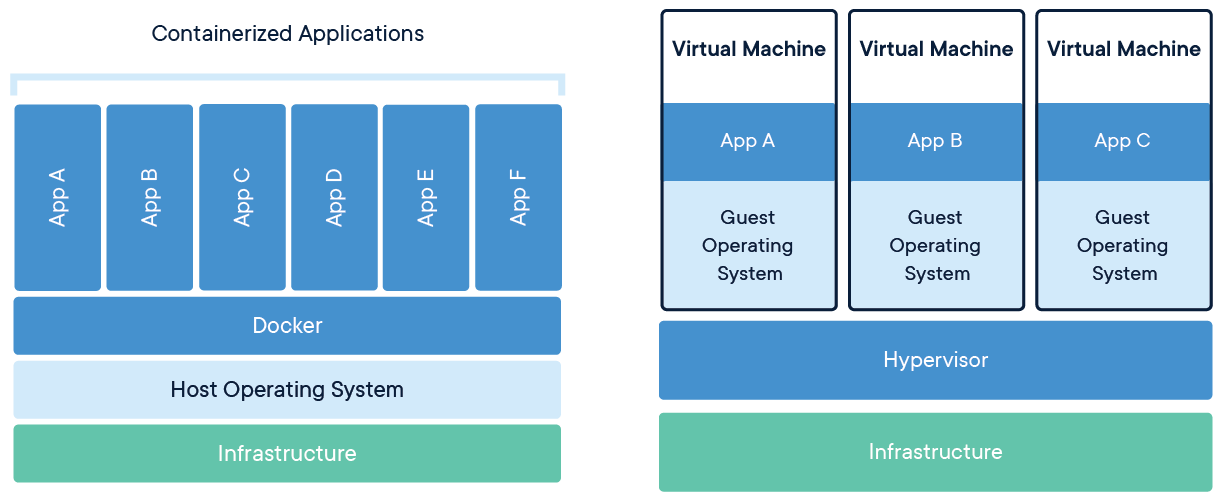
\includegraphics[width=\textwidth]{imagenes/cap4/docker-container.png}
    \caption{Contenedores}
    \label{fig:container_diagram}
\end{figure}


\subsection{Imagen de contenedor}

Una imagen de contenedor es el sistema de archivos aislados de todos los archivos necesarios para ejecutar la aplicación, así como dependencias, configuraciones, ejecutables, etc. Así como también variables de entorno y datos necesarios para ejecutar la aplicación. \cite{Docker}  

\subsection{Redes}

Entre las ventajas de desplegar una aplicación por medio de contenedores Docker es que se pueden comunicar entre ellos y también con servicios externos al entorno de Docker. Por defecto se pueden crear varios tipos de configuraciones de red, pero por lo general se utilizan redes puente entre los contenedores para que estos puedan comunicarse mutuamente entre ellos y solo exponiendo los puertos necesarios para interactuar con el sistema en cuestión y esta es la opción utilizada en nuestra implementación. \cite{Docker}  

\subsection{Volumenes}
Puesto que un contenedor no tiene un estado persistente sobre los datos que genera, se introducen los volúmenes, son la forma recomendada de agregar persistencia de datos a un contendedor de Docker. 
\cite{Docker} 

\begin{figure}[ht]
    \centering
    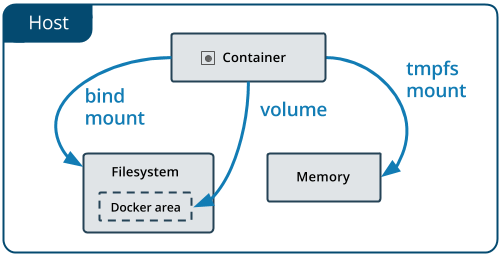
\includegraphics[width=\textwidth]{imagenes/cap4/docker-volume.png}
    \caption{Volumen}
    \label{fig:volume_diagram}
\end{figure}

\subsection{Construción}
Las imágenes de Docker se construyen partir de instrucciones escritas en un archivo denominadado Dockerfile, 
generalmente de parte de una imagen base de la cual sé la adiciona lo necesario para ejecutar la aplicación.
\cite{Docker}


\subsection{Repositorios}
Un repositorio de imágenes Docker(Docker Registry) es un servidor que almacena y distribuye imágenes versionadas generadas partir de un Dockerfile. Estos repositorios pueden ser públicos como DockerHub que es el oficial de la comunidad de Docker como así también privado para un equipo de desarrollo en una institución.
\cite{Docker}

\section{Componentes}

Cada componente del sistema se configuró en un contenedor de Docker con la excepción del servidor NGINX que si estaba instalado sobre el sistema operativo del servidor. 
\begin{figure}[ht]
    \centering
    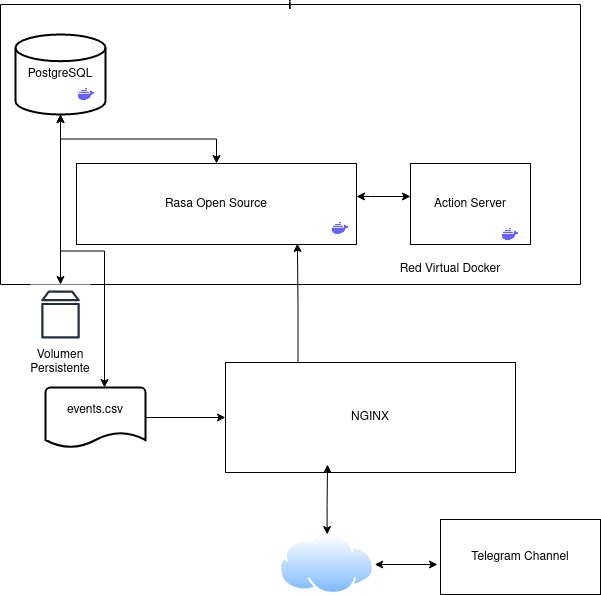
\includegraphics[width=\textwidth]{imagenes/cap4/server.png}
    \caption{Componentes del sistema}
    \label{fig:server_diagram}
\end{figure}


\subsection{Rasa Open Source}

El contendedor de Rasa Open Source ejecuta una imagen oficial proveída por Rasa disponible en los repositorios de DockerHub\cite{DockerHub}, pero con el modelo entrenado y las configuraciones particulares al proyecto. Es el único contenedor que tiene un puerto externo para servir al usuario. También hace uso de los servicios de PosgresSQL y del servicio de acciones(action server). 


\subsection{Servidor de acciones}

Servidor de acciones(acction server) es un servicio interno que ejecuta código escrito en Python este utiliza una imagen oficial para servicios Python disponible en los repositorios de DockerHub\cite{DockerHub}, estos son operaciones específicas para algunas acciones una respuesta no estática, como por el ejemplo la acción relacionada con el cálculo de puntajes en el final desacuerdo a los puntajes en los exámenes parciales.

 \subsection{PostgresSQL}
  
 PostgresSQL es un motor de base de datos del tipo relacional\cite{postgresql} el cual se configuró a partir de una imagen oficial de PostgresSQL disponible en los repositorios de DockerHub\cite{DockerHub}. Aparte de sus funciones de base de datos de sistema, también ejecutar un trabajo periódico(cada una hora) para realizar una copia actualizada de los contenidos de la tabla Eventos a un archivo separado por comas(csv) que se utiliza para retroalimentar las conversaciones y generar más datos para mejorar el modelo. 

 \subsection{NGINX}

 NGINX, es un servidor web que también puede ser usado como proxy reverso, que implica redirigir el tráfico a puertos internos y también para servir archivos que fueron las funciones utilizadas para el proyecto. Así como también puede ser utilizado como balanceador de carga, mail proxy y HTTP cache, entre otras funciones \cite{NGINX}
El servidor NGINX redirige el tráfico a la instancia de Rasa Open Source y si como también sirve el archivo de 
la copia más reciente de la tabla Eventos para agilizar las verificaciones de las respuestas y preguntas recibidas.

\section{Recursos}

Para la puesta en producción del proyecto, se utilizó una instancia de Droplet alojado en Nueva York del proveedor DigitalOcean con un procesador con un 1vcpu(procesador virtualizado), 1 GB de RAM, 25 GB de almacenamiento y con un costo de entre 4 y 6 dólares americanos al mes dependiendo del tráfico presentado. Por las limitaciones de memoria del servidor se configuró también 4 GB de espacio de intercambio(SWAP) en el espacio de almacenamiento.  

\section{Telegram}

Para habilitar pruebas para el público general se eligió Telegram, puesto que es bastante sencillo usar su servicio para conectar a implementaciones de chatbots y este no tiene costo de uso. \cite{botfather}
